% !TEX root = ../thesis.tex

\chapter{AVPipe视频流处理框架的设计与实现}
为了解决在\ref{moti_obj}中所述的目标,我们设计了Accel-Video Pipe(AVPipe),一套模块化的对基于DAG计算图的视频流处理提供开发便捷以及加速优化的编程框架。在这一章中,我们将具体介绍AVPipe的设计逻辑与框架结构。

\section{AVPipe的设计逻辑}
% 先讲逻辑抽象:
%   以 数据流 ,数据处理的分离。由管道将数据与不同处理模块相连接。
% 再讲各部分是如何设计的 
针对视频流处理任务在多阶段有依赖的较复杂计算流程,我们需要使AVPipe编程框架能够对整个智能视频处理流程进行合理的抽象。\par
视频流处理中,数据是不断地由起始节点(source),经过一步步的计算流向汇聚节点(sink)的。这一过程中,数据是在整个计算流程中持续变化的,此外,这些产生的数据也存在着时序上的依赖关系。另一方面,处理流程图中的每一个计算节点所承担的计算任务是固定的。为了对计算流程图进行管理与优化,所有计算模块需要有通过一套简单的、统一的类(class)或结构(struct)来进行封装。\par
基于以上两方面的考虑,我们将AVPipe中的数据与数据处理单元分离开来,分别抽象为StreamPacket和PipeProcessor。为实现数据与数据处理单元之间的交互,我们又建立了对数据流的抽象Stream。数据流(Stream)将不同数据处理单元(PipeProcessor)连接成一个整体,为数据(StreamPacket)提供了流动的载体与指引,使得数据可以有序地、高效地流向各个处理单元。 对数据,数据流以及数据处理单元的抽象是AVPipe框架的主要设计逻辑,图\ref{fig:base_struct}直观展示了这三者在AVPipe中的关系。接下来我们会逐一介绍这三部分的具体设计。
\begin{figure}[htp]
    \centering
    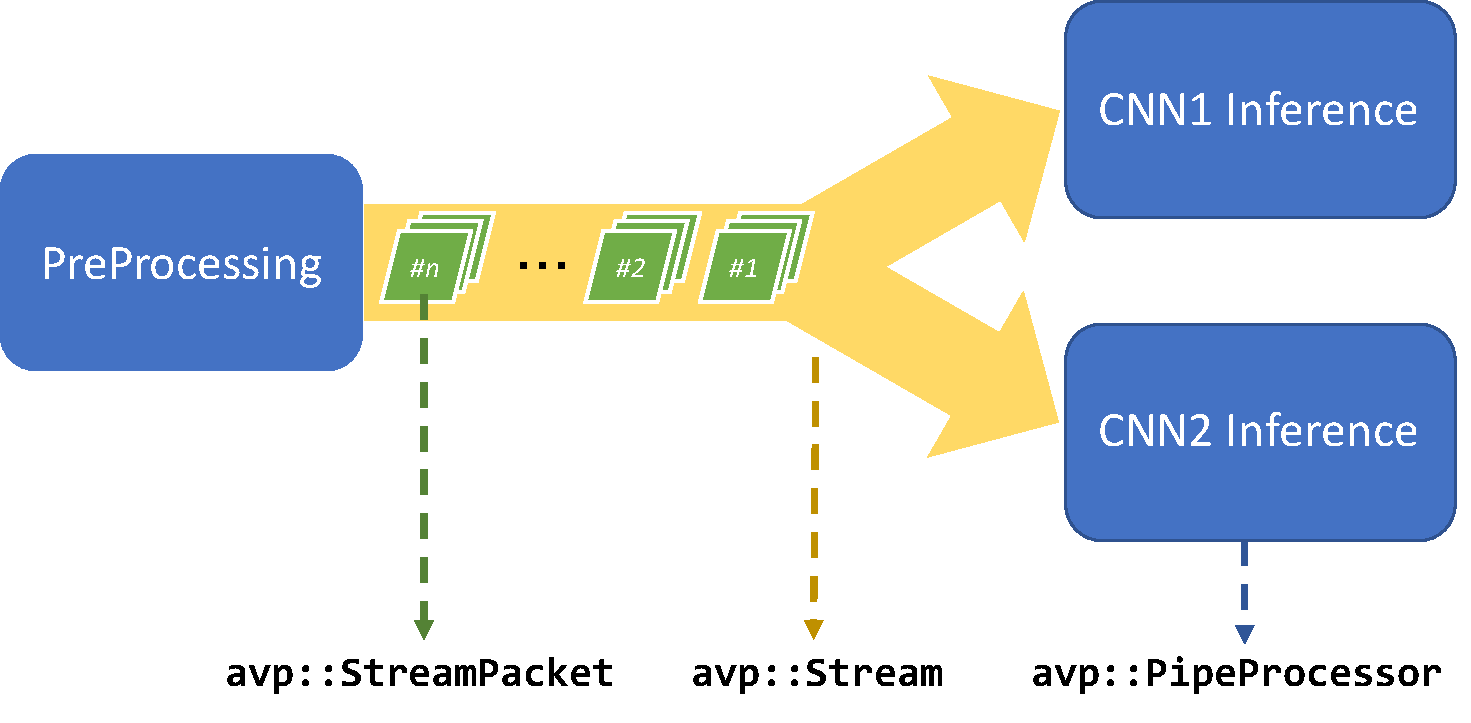
\includegraphics[width=0.8\textwidth]{figure/avp_base_struct.pdf}
    \caption{AVPipe基本抽象之间的关系}
    \label{fig:base_struct}
\end{figure}
\subsection{数据包StreamPacket}
StreamPacket中包含了视频流处理流程中的待处理数据。每个StreamPacket只表示单一类型的数据(如图片,矩阵或张量等)。
为了保证数据的同步与时序,每个StreamPacket都有一个时间戳(timestamp)来记录自己的创建时间步,同一时间步的所有StreamPacket需要在同一处理流程周期中完成。
考虑到某些数据处理步骤可能会在同一时间步中产生多个处理结果,数据在StreamPacket中需要以列表的形式来进行维护。某些数据处理过程也可能会由于没有满足条件而产生空的数据包,空数据包作为作为处理流程中的正常产物,StreamPacket仍然需要对其提供必要的处理逻辑。此外,由于整个AVPipe的数据处理是围绕着StreamPacket来进行的,当整个处理流程结束时,需要依赖StreamPacket的传播来告知每个数据单元来停止运行,因此除了空数据包外,StreamPacket还需提供携带结束信息的终止数据包。
\subsection{数据流Stream}\label{ch4:design_stream}
Stream是StreamPacket的载体,其主体需要存在一个队列结构来有序存取StreamPacket。另一方面,Stream又有着连接PipeProcessor的作用,由于同一个人数据可能会被多个步骤利用,因此同一个Stream可能会同时连接多个PipeProcessor(如图\ref{fig:base_struct})。考虑到多个PipeProcessor可能会多线程同时运行,Stream需要为此提供一定的同步与阻塞机制,以免数据的错位与误读。
当数据包完成在PipeProcessor被使用并完成处理时,PipeProcessor会向Stream发送该数据包的释放请求,Stream要能判断该数据包是否被所连接的所有PipeProcessor全部使用,当且仅当所有PipeProcessor都使用了该数据包后,数据包才会从Stream中安全释放。
有时候,由于数据生产速度会超过数据消费速度,数据包StreamPacket会不断地积累在Stream中而不能及时处理,最终导致大量内存的不必要消耗。为此,Stream还需要提供一个长度或容量的限制,结合阻塞机制来防止数据包的聚积。

\subsection{数据处理单元PipeProcessor}
PipeProcessor是对视频流处理中各个计算步骤的抽象。PipeProcessor从其连接的输入Stream中拿到数据进行处理,将计算结果放入输出Stream中。PipeProcessor根据根据其输入输出的方式不同,可以分为三类:
\begin{enumerate}
    \item 数据处理型(Process):既有输入数据,也有输出数据。视频流处理中的绝大多数多数处理模块的属于这一形式;
    \item 数据起源型(Source):只有输出数据。主要用于获取或产生数据源(如视频摄像头的捕捉或视频文件的读取)供接下来的处理使用;由于Source节点为每一次处理的起点,当视频处理任务结束时,需要由其产生终止数据包来传播给其他所有计算节点。
    \item 数据汇聚型(Sink):只有输入数据。主要用于汇集视频处理的结果,用以保存或窗口展示。当所有的Sink节点都收到终止数据包时,这意味着所有计算节点都收到了终止信号,整个视频处理流程就会停止运行。
\end{enumerate}
流处理中的不同处理模块都是对PipeProcessor的继承与实现。不同模块可以定义自己所需的变量或内存,其实际计算则是通过重载PipeProcessor中的运行接口(\texttt{run})来实现的,在这个运行接口中只需要定义处理相关的计算即可。对于运行的前的准备,输入数据的检查,时间戳的校对则是由PipeProcessor内不另一个接口来实现的(\texttt{process}),\texttt{process}要能检查输入的有效性。当输入为空数据包时,\texttt{process}在默认情况\footnote{部分输入数据为空时,数据处理逻辑也有可能产生非空的输出。如对检测结果的在检测帧上渲染时,检测结果可能为空。}下会直接返回空的输出数据,而不调用\texttt{run}接口。\texttt{process}对终止数据包也会有类似的处理,不再赘述。总之,在实际使用中,我们不能直接调用\texttt{run}的接口,
而是通过调用对\texttt{run}再次封装的\texttt{process}接口。这样的设计一方面可以提高代码运行的可靠性,另一方面可以简化不同模块计算流程的实现。

\section{AVPipe的框架实现}
在介绍了AVPipe主体的设计逻辑后,我们将在本小节关注框架实现中存在的需要特别考虑的内容,同样围绕着数据包,数据流以及数据处理单元这三大部分进行展开。
% 讲 Mat 与 Tensor的 整合
\subsection{StreamPacket中数据格式的整合}
针对\ref{ch3:problems}中提到的数据格式在不同处理步骤中的不能不统一使用的问题,我们期望StreamPacket的封装能够在这方面带来改善。对视频流处理这一类任务来说,我们可以将处理流程中可能涉及到处理数据的格式进行总结。通过调研不同视频流处理任务发现,所涉及的数据处理主要包含两种数据格式:(1)图像的矩阵数据,数据主要以OpenCV的Mat格式来参与传统的数字图像处理运算,如图像的裁剪,缩放,仿射变化等,但是Mat数据有维度的限制,如\ref{ch2:framewk}中所说,它不能很好地处理高维张量数据;(2)机器学习相关的张量数据,张量数据主要用于神经网络的计算以及相关的后处理操作中,张量数据在各个深度学习推理引擎中的表示不尽相同,对高维张量的操作难易程度也不尽相同。通过以上分析,我们可以确定的是StreamPacket需要同时对图像矩阵以及高维张量提供良好的支持,接下来我们要考虑具体实现实现方式。\par

首先,在关于图像矩阵的处理上,OpenCV是受业界普遍认可的通用数字图像处理库。因此,在StreamPacket中的数据提供直接的\texttt{cv::Mat}形式的数据存储是对传统数字图像处理操作最友好的支持。
再来看对高维张量的处理。由于这方面的需求是在近些年由机器学习技术的快速发展而兴起的,这使得目前在C/C++语言下没有一个像Python中NumPy那样的,开发完善的,普遍使用的针对高维数据的科学计算库,从而导致不同的机器学习框架会各自为阵,开发仅供本框架使用的数据格式以及数据处理方式,如TVM所使用的DLPack\cite{dlpack}库,PyTorch所使用的ATen库。通过实际使用和测试发现,PyTorch/Caffe2所使用的ATen张量库有最为完善的张量定义以及操作算子,其类似Python的数据操作与丰富的开发文档也带来了出色的使用体验。我们也因此将ATen库中的张量格式\texttt{at::Tensor}做为AVPipe主要支持的张量格式。\par

通过以上分析,我们确立了对\texttt{cv::Mat}以及\texttt{at::Tensor}这两种数据格式的支持,我们现在开始考虑如何对这两部分在StreamPacket中进行有机结合。考虑到OpenCV与LibTorch都是提供预编译的开源库,我们并不打算对这两个库的底层代码进行修改以实现操作的互通,这在工程难度以及通用性上都不可行。于是我们考虑在StreamPacket中同时保留\texttt{Mat}和\texttt{Tensor}的数据队列。通常情况下,一个Stream对应的StreamPacket都是同一个类型的,也就是说,\texttt{Mat}和\texttt{Tensor}两者中一般只有一个保存有待处理数据。PipeProcessor在生成数据时,也会规定数据将在StreamPacket中以哪种方式保存,这使得StreamPacket在管理内部数据时只需关注它所对应形式的数据。
此外,我们也在StreamPacket的内部,通过内存指针引用的方式,提供了\texttt{Mat}和\texttt{Tensor}相互类型转换的方法,为不同应用场景提供便利。

% 同步以及其他特殊情况的考虑
\subsection{Stream中数据的同步与管理}
在\ref{ch4:design_stream}中,我们介绍了Stream的设计逻辑。在这一部分里,我们主要说明在Stream实现过程中要考虑的关键点。由于Stream本质是存放AVPipe数据包的一个队列,因此Stream直接继承STL(C++标准模版库)中的deque\footnote{\url{http://www.cplusplus.com/reference/deque/deque/}},并在此基础上提供功能的完善与拓展。\par

对deque拓展的核心在于为其添加多线程的数据同步与阻塞机制,在这里我们使用C++11标准提供的多线程相关函数库来进行实现。 

% 数据如何在多个计算库运转与整合
\subsection{多种计算库的支持方式}
% Processor 的实现与自定义
\subsection{计算模块的实现与自定义}


\section{AVPipe的自动化工具}

\subsection{配置文件驱动的自动代码生成}

\subsection{运行时性能分析驱动的自动多线程优化}

\subsection{异构场景下的计算资源分配与调度}

